\chapter{Arhitektura i dizajn sustava}
		
		Arhitektura ovog sustava je bazirana na arhitekturi klijent-poslužitelj. Sustav se sastoji od 3 sloja: sloj korisničkog sučelja, sloj aplikacijske logike, sloj podataka.
		
		\textbf{Web preglednik} je program preko kojeg korisnik koristi aplikaciju. Preglednik omogućuje klijentu komunikaciju s web poslužiteljem aplikacije. Preglednik nam omogućava prikaz sloja korisničkog sučelja sustava. Korisnik preko web preglednika komunicira s web poslužiteljem slanjem i primanjem HTTP zahtjeva. Primljene podatke i datoteke web preglednik zna interpretirati i prikazati korisniku tako da sama interakcija s aplikacijom bude jednostavna. Neki od popularnih web preglednika su Crome, Safari i Edge.
		
		\textbf{Web poslužitelj} je računalo na kojem se aplikacija pokreće. Na njemu se dakle nalazi sloj aplikacijske logike. Web poslužitelj aplikaciji prosljeđuje zahtjeve na obradu i njezine odgovore prosljeđuje natrag klijentima. Web aplikacija na poslužitelju obrađuje zaprimljene zahtjeve. Ako obrada zahtjeva to zahtjeva, web aplikacija dodatno komunicira sa slojem podataka.
		
		\textbf{Baza Podataka} predstavlja sloj podataka. U bazi podataka se na siguran način spremaju svi podaci koje je potrebno trajno čuvati. To podrazumijeva podatke o prijavama, korisničkim računima i slično. Takvi podaci moraju ostati očuvani i ako je rad aplikacije prekinut iz bilo kojeg razloga. Baza podataka je detaljnije opisana u poglavlju  \ref{sec:bazaPodataka}.
		
		\textbf{Web aplikacija} je podijeljena na frontend i backend.
		
		\textbf{Frontend} je zapravo prezentacijski dio aplikacije i zadužen je za interakciju s korisnikom. On oblikuje korisničko sučelje i samim time definira što će korisnik vidjeti na web pregledniku kada koristi aplikaciju.
		
		\textbf{Backend} je dio aplikacije koji obrađuje zahtjeve i kontrolira rad ostalih dijelova sustava. Baceknd je usko povezan s web poslužiteljem.
		
		Za izradu backend dijela aplikacije odabrali smo programski jezik Java s radnim okvirom Spring Boot. Spring Boot radni okvir koristi višeslojnu arhitekturu u kojoj svaki sloj komunicira sa slojem koji se u hijerarhiji nalazi iznad ili ispod njega. Arhitektura Spring Boota se sastoji od četiri sloja:
		\begin{packed_item}
			\item \textbf{Prezentacijski sloj} (\textit{Presentation layer}) - Ovo je najviši sloj arhitekture i predstavlja frontend dio aplikacije. Ovaj sloj prima HTTP zahtjeve i vrši autentifikaciju. Također vrši pretvorbu JSON objekata u objekte u Javi i obrnuto. Na kraju svoje obrade Prezentacijski sloj prosljeđuje HTTP zahtjev sljedećem sloju.
			
			\item \textbf{Poslovni sloj} (\textit{Business layer}) - Ovaj sloj sadrži svu poslovnu logiku te je zadužen za validaciju i autorizaciju.
			
			\item \textbf{Sloj postojanosti} (\textit{Persistence layer}) - Ovaj sloj sadrži logiku vezanu uz pohranu u bazu podataka. Sloj pretvara zapise iz baze podataka u objekte iz poslovnog sloja i obrnuto.
			
			\item \textbf{Sloj baze podataka} (\textit{Database layer}) - Ovaj sloj sadrži bazu podataka ili više njih. Sloj je zadužen za obavljanje CRUD (copy, read, update, delete) operacija.
		\end{packed_item}
		
		\begin{figure}[H]
			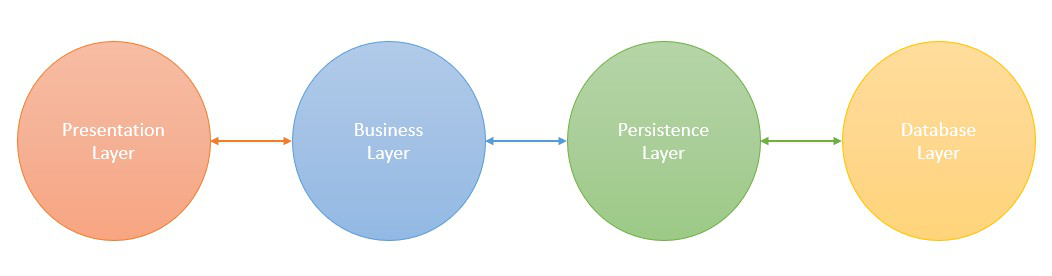
\includegraphics[width=\textwidth]{slike/slojeviArhitekture.jpg} %veličina u odnosu na širinu linije
			\caption{Prikaz Spring Boot arhitekture}
			\label{fig:MVC1} %label mora biti drugaciji za svaku sliku
		\end{figure}
		
		Za razvoj frontend dijela aplikacije odlučili smo koristiti programski jezik JavaScript uz radni okvir React. React omogućuje jednostavnu izradu korisničkog sučelja preko JavaScripta, bez direktnog korištenja HTML-a.
		
		Za razvojne okoline smo odlučili koristiti IntelliJ IDEA za rad u Spring Boot radnom okviru i Visual Studio Code za rad u React radnom okviru.
		
	\eject
	
		\section{Baza podataka}
		\label{sec:bazaPodataka}
		
		Ovaj sustav će za svoje potrebe koristiti relacijsku bazu podataka implementirana u PostgreSQL-u. Ovakav tip baze podataka svojom strukturom omogućuje jednostavno modeliranje elemenata iz stvarnog svijeta i zbog toga je široko primjenjiv. Odabrali smo implementaciju u PostgreSQL-u jer smo s ovom implementacijom već dobro upoznati. Relacijske baze podataka se sastoje od relacija. Relacije su predstavljene tablicama koje su definirane svojim nazivom i skupom atributima. Bazu podataka koristimo za jednostavnu i sigurnu pohranu, izmjenu, umetanje i dohvat podataka potrebnih za rad sustava. Naša baza podataka se sastoji od sljedećih relacija, odnosno tablica:
		
		\begin{packed_item}
			\item Users
			\item Report
			\item Image
			\item Category
			\item CategoryKeywords
			\item ReportGroup 
			\item Feedback
			\item CityOffice
		\end{packed_item}
		
		S obzirom na to da je još u fazi razvoja, aplikacija trenutno koristi H2 bazu podataka u radnoj memoriji. Ovu bazu podataka Spring Boot automatski inicijalizira i spaja s aplikacijom. Ova baza je pogodna za testiranje i razvoj te smo je zbog toga odlučili koristiti tijekom razvoja. Kasnije kada aplikacija bude gotova ćemo H2 bazu zamijeniti odvojenom PostgreSQL bazom podataka.
		
			\subsection{Opis tablica}
			
			\textbf{Users} tablica čuva podatke o korisničkim računima koje korisnici izrađuju tijekom registracije. Tablica je povezana vezom \textit{One-to-Many} s tablicom \textit{Report} preko atributa \textit{userID}.
			
			\begin{longtblr}[
					label=Users,
					entry=none
				]{
					width = \textwidth,
					colspec={|X[6,l]|X[6, l]|X[20, l]|}, 
					rowhead = 1,
				} %definicija širine tablice, širine stupaca, poravnanje i broja redaka naslova tablice
				\hline \SetCell[c=3]{c}{\textbf{Users}}	 \\ \hline[3pt]
				\SetCell{LightGreen} userID & INT & jedinstveni identifikator korisnika \\ \hline
				email & VARCHAR & email adresa korisnika \\ \hline 
				firstName & VARCHAR & ime korisnika \\ \hline
				lastName & VARCHAR & prezime korisnika \\ \hline 
				password & VARCHAR & kriptirana lozinka za korisnički račun \\ \hline 
			\end{longtblr}
			
			\textbf{Report} tablica čuva podatke o pojedinim prijavama oštećenja koje korisnici podnose. Tablica je povezana vezom \textit{Many-to-One} s tablicom \textit{Users} preko atributa \textit{userID}, \textit{Many-to-One} vezom s tablicom \textit{Category} preko atributa \textit{categoryID}. Također postoji auto-refleksivna \textit{Many-to-One} veza kojom se modelira nadovezivanje prijava.
			
			\begin{longtblr}[
				label=Report,
				entry=none
				]{
					width = \textwidth,
					colspec={|X[8,l]|X[6, l]|X[20, l]|}, 
					rowhead = 1,
				} %definicija širine tablice, širine stupaca, poravnanje i broja redaka naslova tablice
				\hline \SetCell[c=3]{c}{\textbf{Report}}	 \\ \hline[3pt]
				\SetCell{LightGreen} reportID & INT & jedinstveni identifikator prijave \\ \hline
				location & VARCHAR & lokacija oštećenja \\ \hline
				description & VARCHAR & opis oštećenja \\ \hline 
				reportTS & TIMESTAMP & vrijeme prijave \\ \hline 
				reportHeadline & VARCHAR & naslov prijave \\ \hline 
				\SetCell{LightBlue} userID & INT & jedinstveni identifikator korisnika koji je podnio prijavu \\ \hline 
				\SetCell{LightBlue} categoryID & INT & jedinstveni identifikator kategorije oštećenja \\ \hline
				\SetCell{LightBlue} isConnectedToID & INT & jedinstveni identifikator prijave na koju je ova prijava nadovezana \\ \hline
			\end{longtblr}
			
			\textbf{Image} tablica čuva podatke o slikama koje se prilažu u prijavama oštećenja. Tablica je povezana \textit{Many-to-One} vezom s tablicom \textit{Report} preko atributa \textit{reportID}.
			
			\begin{longtblr}[
				label=Image,
				entry=none
				]{
					width = \textwidth,
					colspec={|X[6,l]|X[6, l]|X[20, l]|}, 
					rowhead = 1,
				} %definicija širine tablice, širine stupaca, poravnanje i broja redaka naslova tablice
				\hline \SetCell[c=3]{c}{\textbf{Image}}	 \\ \hline[3pt]
				\SetCell{LightGreen} imageID & INT & jedinstveni identifikator slike \\ \hline
				\SetCell{LightBlue} reportID & INT & jedinstveni identifikator prijave kojoj slika pripada \\ \hline
				URL & VARCHAR & URL slike \\ \hline 
			\end{longtblr}
			
			\textbf{Category} tablica čuva podatke o kategorijama kojima oštećenje može pripadati. Tablica je povezana \textit{One-to-Many} vezom s tablicom \textit{Report} preko atributa \textit{categoryID}, \textit{Many-to-One} vezom s tablicom \textit{CityOffice} preko atributa \textit{cityOfficeID} i \textit{One-to-Many} vezom s tablicom \textit{CategoryKeywords} preko atributa \textit{categoryID}.
			
			\begin{longtblr}[
				label=Category,
				entry=none
				]{
					width = \textwidth,
					colspec={|X[6,l]|X[6, l]|X[20, l]|}, 
					rowhead = 1,
				} %definicija širine tablice, širine stupaca, poravnanje i broja redaka naslova tablice
				\hline \SetCell[c=3]{c}{\textbf{Category}}	 \\ \hline[3pt]
				\SetCell{LightGreen} categoryID & INT & jedinstveni identifikator kategorije \\ \hline
				categoryName & VARCHAR & naziv kategorije \\ \hline 
				\SetCell{LightBlue} cityOfficeID & INT & jedinstveni identifikator gradskog ureda koji obrađuje prijave oštećenja iz ove kategorije \\ \hline
			\end{longtblr}

			\textbf{CategoryKeywords} tablica čuva podatke o ključnim riječima po kojima se može identificirati kategorija oštećenja. Tablica je povezana \textit{Many-to-One} vezom s tablicom \textit{Category} preko atributa \textit{categoryID}.

			\begin{longtblr}[
				label=CategoryKeywords,
				entry=none
				]{
					width = \textwidth,
					colspec={|X[6,l]|X[6, l]|X[20, l]|}, 
					rowhead = 1,
				} %definicija širine tablice, širine stupaca, poravnanje i broja redaka naslova tablice
				\hline \SetCell[c=3]{c}{\textbf{CategoryKeywords}}	 \\ \hline[3pt]
				\SetCell{LightGreen} keywordID & INT & jedinstveni identifikator ključne riječi \\ \hline
				keyword & VARCHAR & ključna riječ \\ \hline 
				\SetCell{LightBlue} categoryID & INT & jedinstveni identifikator kategorije kojoj ključna riječ pripada. \\ \hline
			\end{longtblr}
			
			\textbf{Feedback} tablica čuva podatke o statusu prijava koje su povezane. Također čuva podatke potrebne za slanje povratnih informacija korisnicima i računanje nekih statistika. Tablica je povezana \textit{Many-to-One} vezom s tablicom \textit{Report} preko atributa \textit{reportID}.
			
			\begin{longtblr}[
				label=Feedback,
				entry=none
				]{
					width = \textwidth,
					colspec={|X[6,l]|X[6, l]|X[20, l]|}, 
					rowhead = 1,
				} %definicija širine tablice, širine stupaca, poravnanje i broja redaka naslova tablice
				\hline \SetCell[c=3]{c}{\textbf{Feedback}}	 \\ \hline[3pt]
				\SetCell{LightGreen} reportID & INT & jedinstveni identifikator grupe prijava na koju se podaci referiraju \\ \hline
				\SetCell{LightGreen} status & VARCHAR & status prijava u referiranoj grupi \\ \hline 
				changeTS & TIMESTAMP & vrijeme kada se postavio status prijava iz referirane grupe \\ \hline
			\end{longtblr}
			
			\textbf{CityOffice} tablica čuva podatke o računima gradskih ureda. Tablica je povezana \textit{One-to-Many} vezom s tablicom \textit{Feedback} preko atributa \textit{cityOfficeID} i \textit{One-to Many} vezom s tablicom \textit{Category} preko atributa \textit{cityOfficeID}.
			
			\begin{longtblr}[
				label=CityOffice,
				entry=none
				]{
					width = \textwidth,
					colspec={|X[10,l]|X[6, l]|X[20, l]|}, 
					rowhead = 1,
				} %definicija širine tablice, širine stupaca, poravnanje i broja redaka naslova tablice
				\hline \SetCell[c=3]{c}{\textbf{CityOffice}}	 \\ \hline[3pt]
				\SetCell{LightGreen} cityOfficeID & INT & jedinstveni identifikator gradskog ureda \\ \hline
				cityOfficeName & VARCHAR & naziv gradskog ureda \\ \hline
				cityOfficeEmail & VARCHAR & email adresa gradskog ureda \\ \hline 
				cityOfficePassword & VARCHAR & kriptirana lozinka za račun gradskog ureda \\ \hline
			\end{longtblr}
			
			\subsection{Dijagram baze podataka}
			
			\begin{figure}[H]
				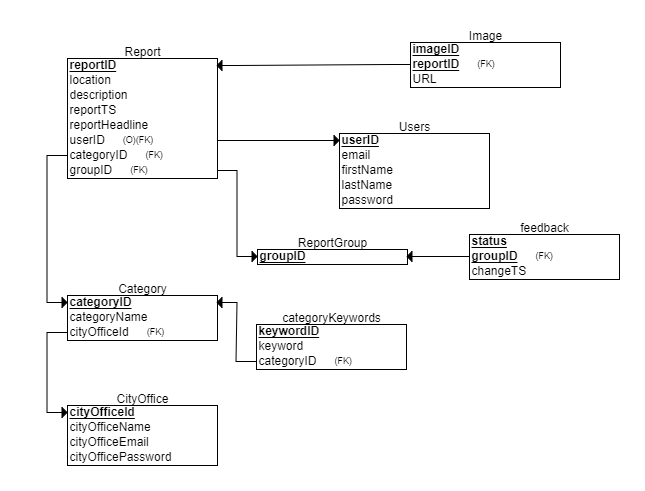
\includegraphics[width=\textwidth]{slike/relacijski.png} %veličina u odnosu na širinu linije
				\caption{Relacijski dijagram baze podataka}
				\label{fig:DijagramBazePodataka} %label mora biti drugaciji za svaku sliku
			\end{figure}
			
			\eject
			
			
		\section{Dijagram razreda}
		
			Na slikama \ref{fig:kontroler}, \ref{fig:dao}, \ref{fig:repo}, \ref{fig:service} su prikazani razredi koji pripadaju backend dijelu aplikacije. Razredi su arhitekturom podijeljeni na kontrolere, repozitorije i servise. Također postoje Domain i DTO (Data Transfer Object) modeli. Svi dijagrami su podložni promjenama, s obzirom na to da je aplikacija još uvijek u fazi razvoja.
		
			Slika \ref{fig:kontroler} prikazuje klase koje imaju ulogu kontrolera, tj. u kodu imaju anotaciju @RestController. Te klase definiraju endpointove i koriste se za dohvat i manipuliranje podacima iz baze podataka. ClientForwardController je kontroler koji povezuje Spring server React aplikacijom. Klase sa @RestController anotacijom koriste instance servisa. Servisi su klase koje imaju @Service anotaciju. Servisi implementiraju metode za upis (npr. createUser(Users);, createCitiyOffice(cityOffice), itd.), brisanje, dohvat i izmjenu podataka u bazi. Klasa ServerApplication je glavna klasa koja pokreće aplikaciju, a ServerApplicationTest služi za testiranje funkcionalnosti aplikacije, ali još nema implementiranu nikakvu funkcionalnost.
		
			\begin{figure}[H]
				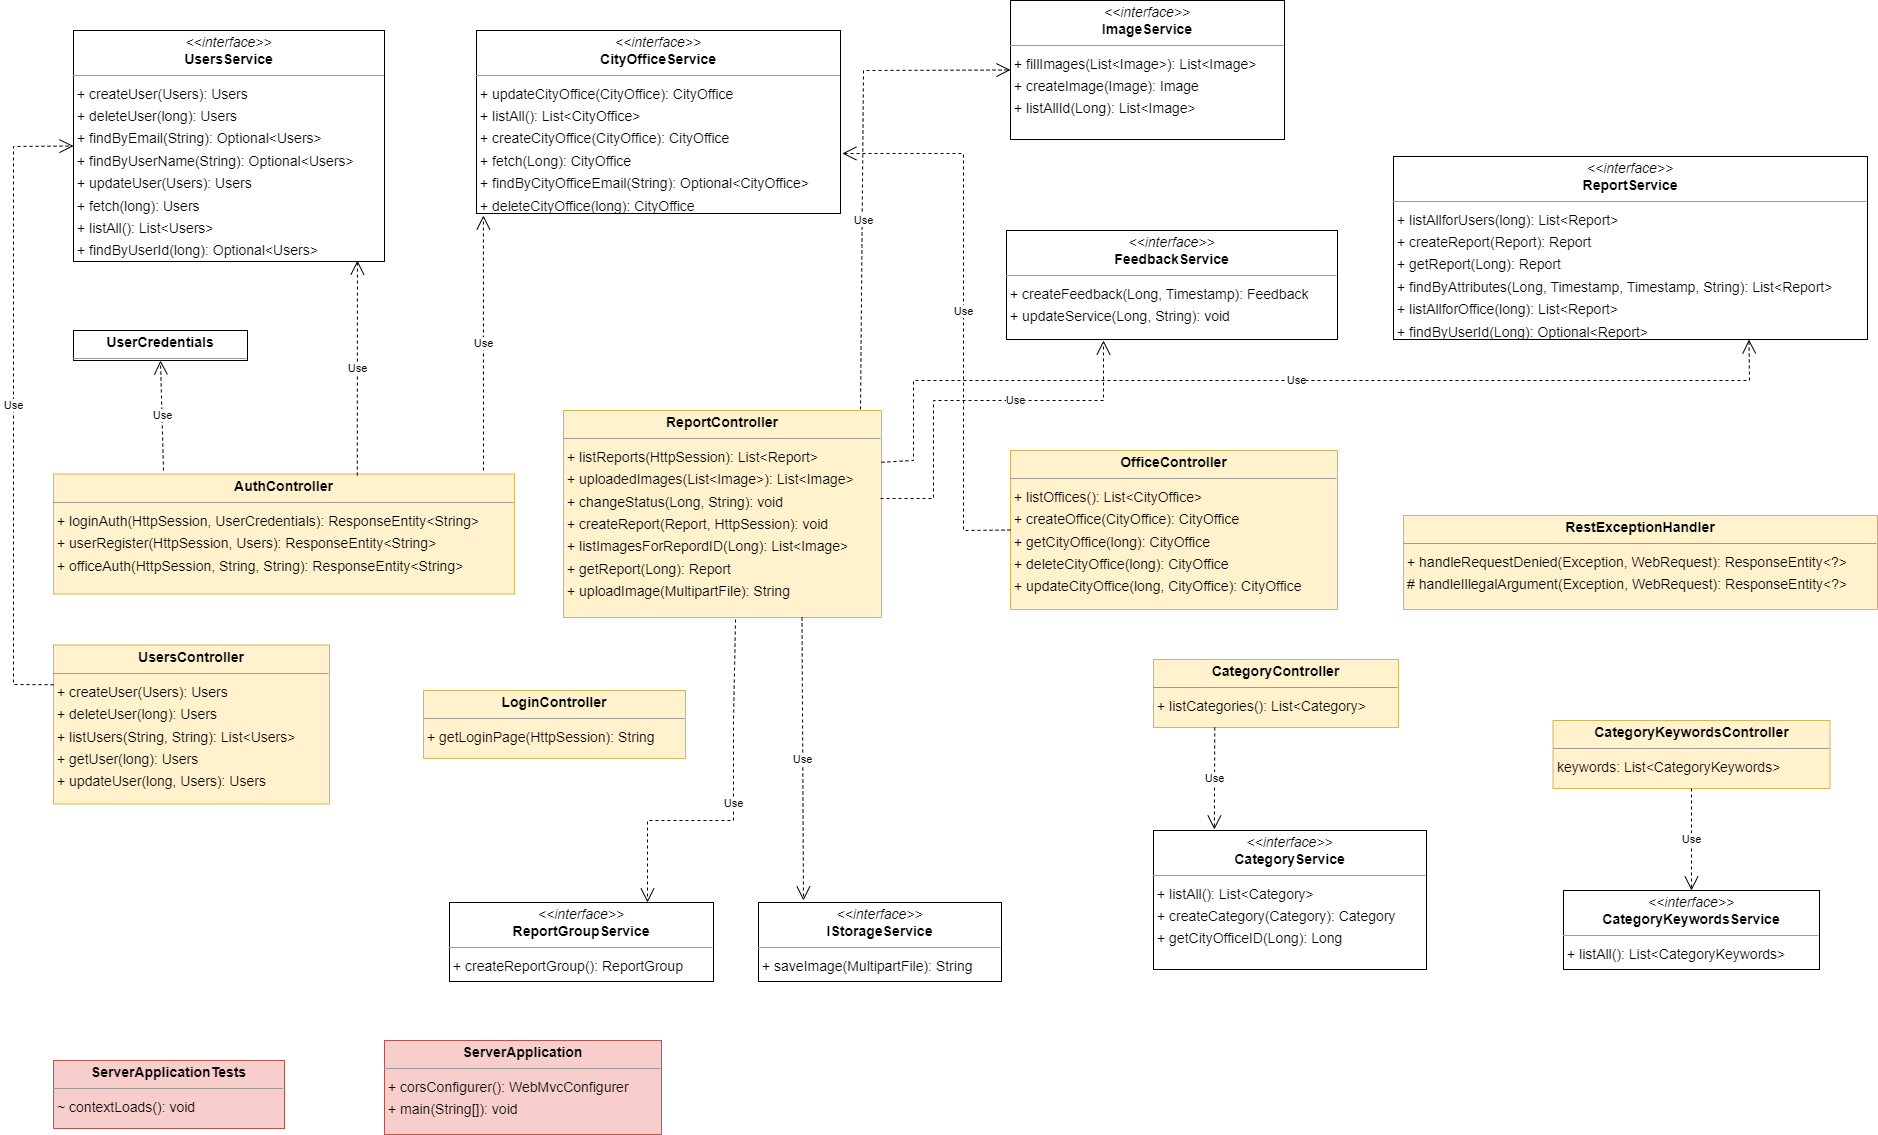
\includegraphics[width=\textwidth]{slike/controller.png} %veličina u odnosu na širinu linije
				\caption{Kontroleri na backendu}
				\label{fig:kontroler} %label mora biti drugaciji za svaku sliku
			\end{figure}
			
			\eject
			
			Slika \ref{fig:dao} prikazuje sučelja koja nasljeđuju sučelje JpaRepository. Sučelje JpaRepository definira razne CRUD (create, read, update, delete) metode za rad nad entitetima u bazi. Definirane metode izvršavaju razne vrste upite nad bazom podataka.
			
			\begin{figure}[H]
				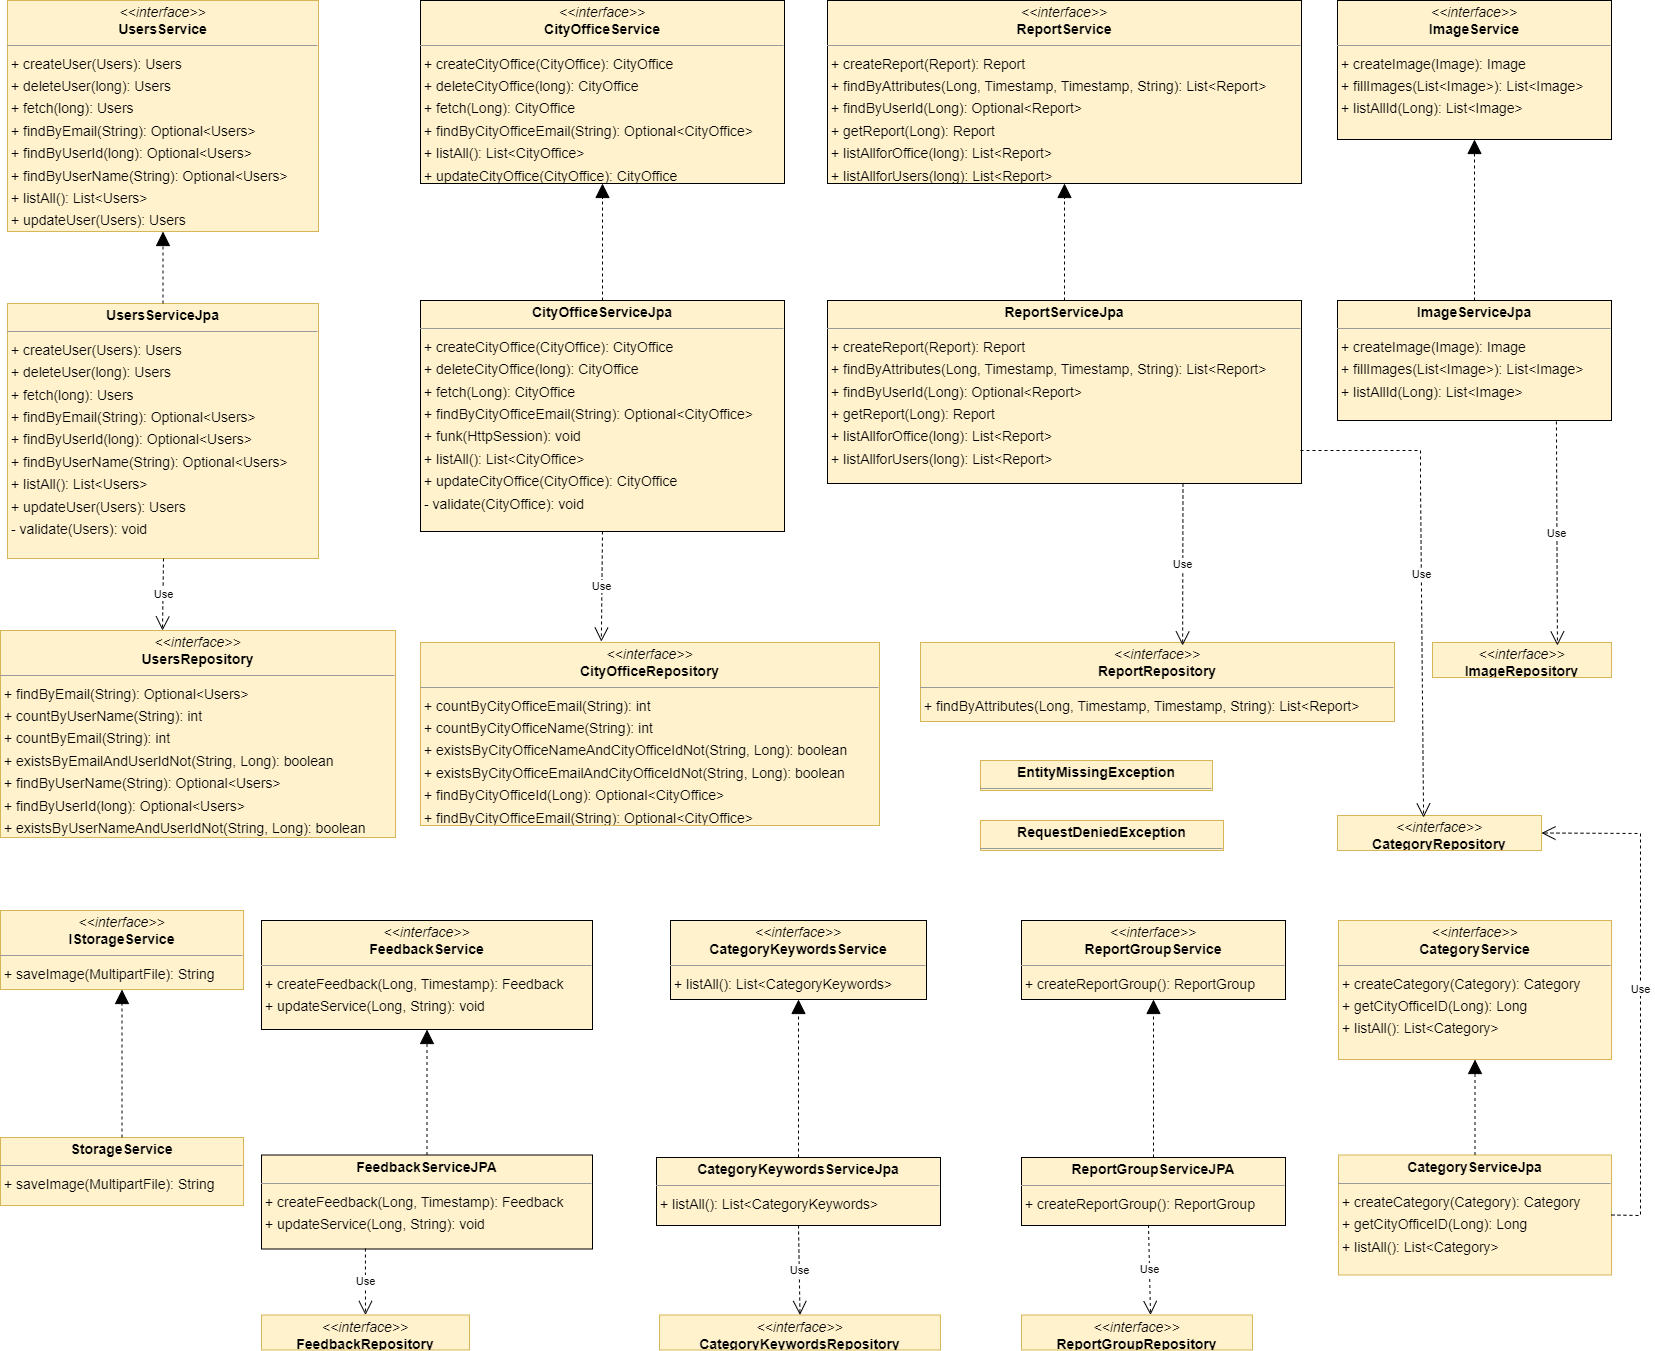
\includegraphics[width=\textwidth]{slike/dao.png} %veličina u odnosu na širinu linije
				\caption{Data Access Objects}
				\label{fig:dao} %label mora biti drugaciji za svaku sliku
			\end{figure}
			
			\eject
			
			Slika \ref{fig:repo} prikazuje klase u paketu repo koje reprezentiraju entitete u bazi podataka te njihove međusobne veze. Ove klase definiraju tipove atributa pojedinih entiteta, ograničenja nad atributima i primarne i strane ključeve. Svaka klasa ima implementirane metode get() i set() za svaki od atributa, kao i odgovarajuće konstruktore. Klasa FeedbackID služi kao pomoćna klasa za definiranje primarnog ključa feedback. Korisnici (Users) stvaraju prijave (Report), a gradski uredi (CityOffice) upravljaju prijavama i prilikom promjena automatski zapisuje nove povratne informacije (Feedback) u bazu podataka za tu grupu prijava.
			
			\begin{figure}[H]
				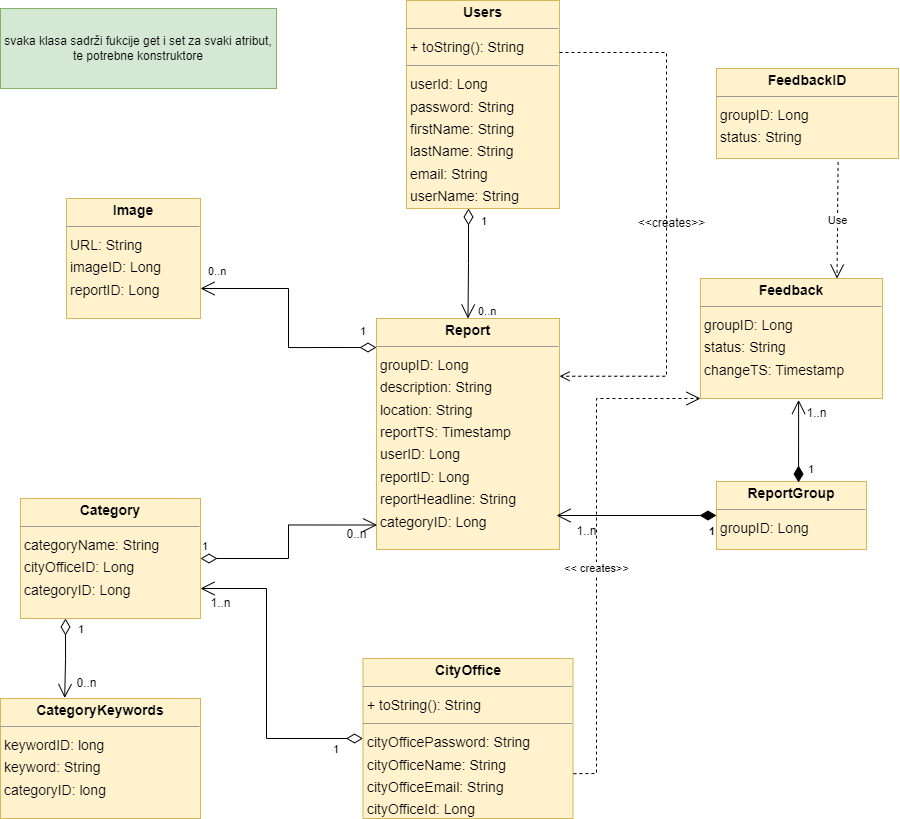
\includegraphics[width=\textwidth]{slike/repo.png} %veličina u odnosu na širinu linije
				\caption{Modeli}
				\label{fig:repo} %label mora biti drugaciji za svaku sliku
			\end{figure}
			
			\eject
			
			Slika \ref{fig:service} prikazuje klase servisa koje definiraju metode za CRUD operacije nad bazom podataka. EntityMissingException i RequestDeniedException su pomoćne klase za baratanje pogreškama. Klase servisa koriste instance Repository klasa iz slike 2. za poziv metoda definiranih u sklopu sučelja Repository odnosno JpaRepository.
			
			\begin{figure}[H]
				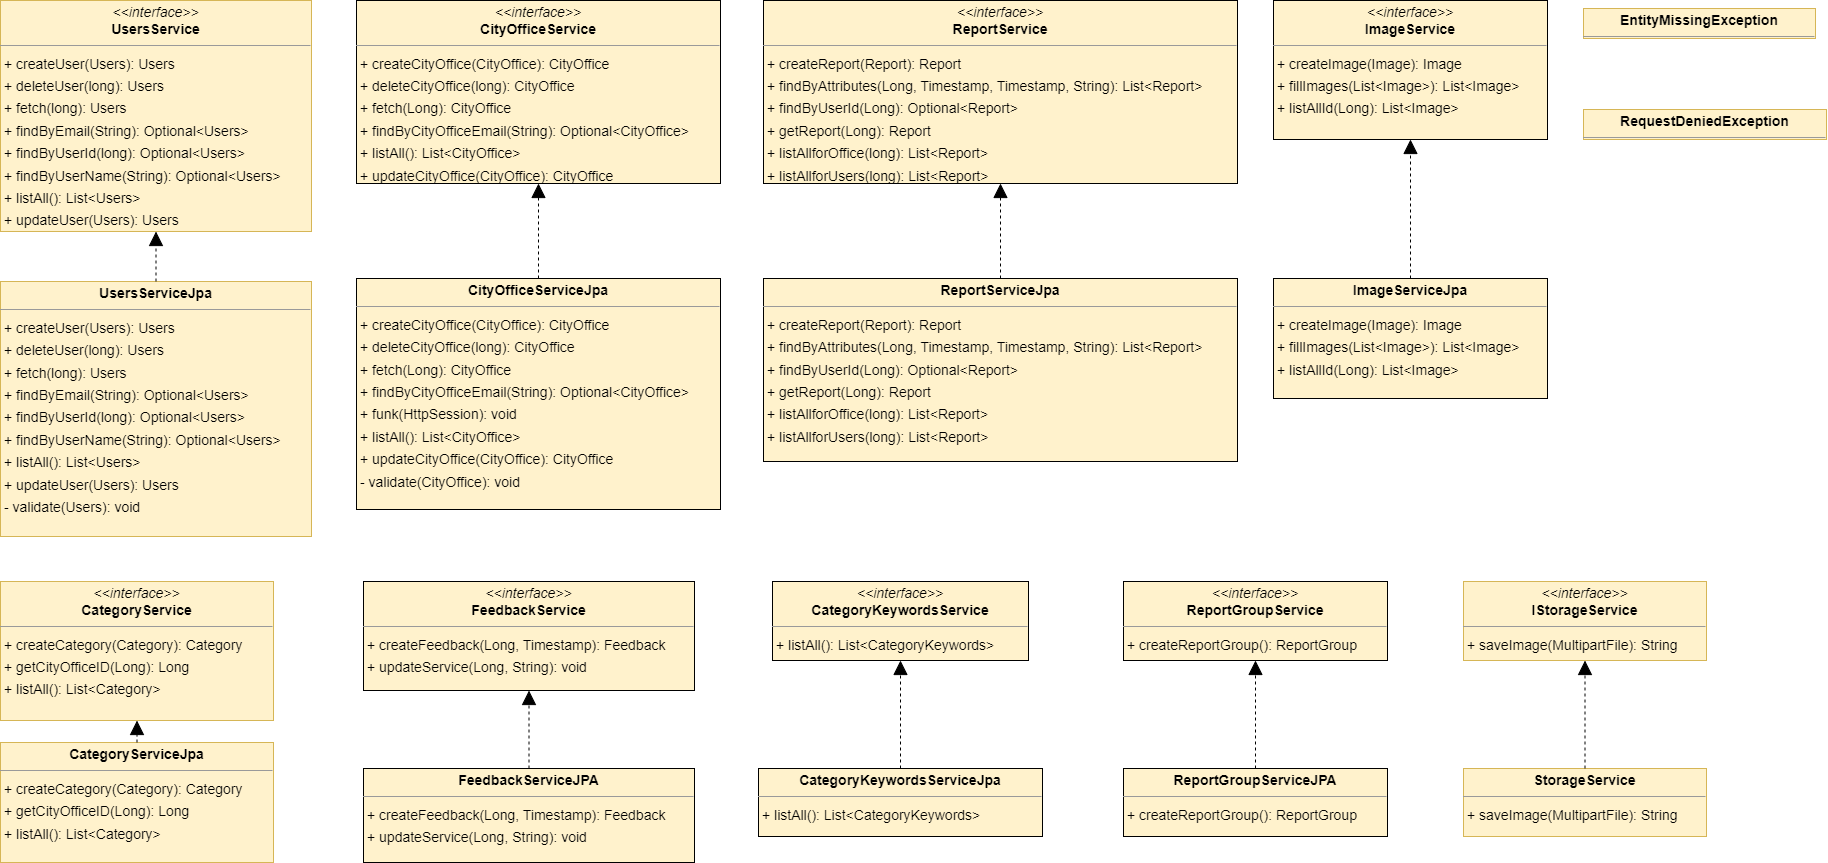
\includegraphics[width=\textwidth]{slike/service.png} %veličina u odnosu na širinu linije
				\caption{Servisi}
				\label{fig:service} %label mora biti drugaciji za svaku sliku
			\end{figure}
			
			\eject
			
			
			\section{Dijagram stanja}
			
			Dijagram stanja je vrsta UML dijagrama koja prikazuje stanja objekta i prijelaze između stanja. Prijelazi se aktiviraju određenim događajima i opcionalno dodatnim uvjetima. 
			
			Slika \ref{fig:dijagramStanja} prikazuje dijagram stanja za korisnika koji može, ali i ne mora biti prijavljen u sustav. 
			
			Korisniku je na početku prikazana glavna stranica na kojoj je karta sa prikazanim aktivnim prijavama u sustavu. Zaglavlje stranice sadrži gumbove za podnošenje nove prijave oštećenja ("Prijava štete"), prikaz statistike prijava ("Statistika"). Također, zaglavlje sadrži gumb sa e-mailom korisnika koji služi za upravljanje korisničkim računom ako je korisnik prijavljen u sustav. Ako korisnik nije prijavljen, zaglavlje sadrži gumbove za prijavu ("Log in") i registraciju ("Register") u  sustav. S obzirom da je zaglavlje isto na svim dijelovima aplikacije, korisnik ima pristup ovim opcijama bilo gdje u aplikaciji.
			
			Na glavnoj stranici korisnik može odabrati filtar prijava. Pomoću tog filtra korisnik može filtrirati aktivne prijave u sustavu koje će se prikazati na karti na početnoj stranici. Odabirom neke od prikazanih prijava na karti korisniku se otvara stranica odabrane prijave. Ako je ta prijava nadovezana na drugu prijavu oštećenja, korisnik može kliknuti na tu prijavu da mu se otvori stranica nadprijave.
			
			Kod pregleda statistike prijava korisnik mora ispuniti obrazac filtra. Nakon potvrde obrasca korisniku se prikazuje statistika prijava koje su odabrane pomoću filtra. 
			
			Prilikom prijave novog oštećenja korisnik ispunjava obrazac prijave. Kada je u obrazac upisan opis oštećenja, sustav korisniku predlaže kategoriju oštećenja. Kada korisnik podnese prijavu, sustav provjerava ako već postoji slična prijava. Ako postoji, sustav nudi korisniku nadovezivanje njegove prijave na postojeću. Korisnik to može prihvatiti, ali može i poslati nepovezanu prijavu. Nakon konačnog podnošenja prijave sustav korisniku prikazuje jedinstveni kod prijave. Korisnik se vraća na početnu stranicu kada potvrdi zaprimljeni kod prijave.
			
			Ako je korisnik prijavljen može pregledati podatke o svojem korisničkom računu. Prilikom pregleda korisničkog računa može dodatno pregledavati vlastite prijave. Kada želi pregledati neku od prijava, korisniku se prikazuje stranica te prijave, isto kao i kod pregleda svih prijava na početnoj stranici. Korisnik također može mijenjati podatke o svojem korisničkom računu. Kod potvrde se izmjene spremaju, ako je do njih došlo. Također, korisnik kod pregleda računa može izbrisati svoj račun čime on postaje neprijavljen i neregistriran.
			
			\begin{figure}[H]
				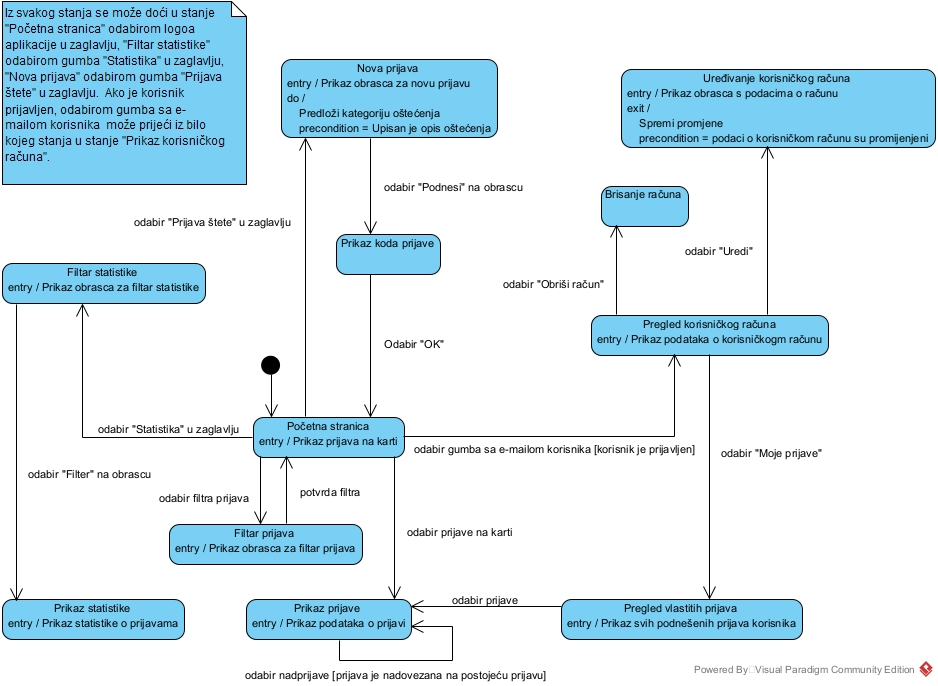
\includegraphics[width=\textwidth]{slike/dijagramStanja.jpg} %veličina u odnosu na širinu linije
				\caption{Dijagram stanja}
				\label{fig:dijagramStanja} %label mora biti drugaciji za svaku sliku
			\end{figure}
			
			\eject 
			
			\section{Dijagram aktivnosti}
			
			Dijagram aktivnosti je ponašajni UML dijagram koji modelira ponašanje sustava nizom akcija koje zajedno čine aktivnost. Dijagram aktivnosti se primjenjuje za modeliranje upravljačkog i podatkovnog toka. Ovakav tip dijagrama nije preporučljiv za modeliranje sustava sa događajima poticanim ponašanjem. Kod dijagrama aktivnosti svaka akcija se izvršava nakon završavanja prethodne akcije. Općenito je u dijagramu aktivnosti naglasak na jednostavnosti prikaza.
			
			Na dijagramu \ref{fig:dijagramAktivnosti} prikazan je proces podnošenja prijave oštećenja i njezine obrade u gradskom uredu. 
			
			Korisnik odabire opciju "Prijava štete" te ispunjava podatke o oštećenju na dobivenom obrascu. Kada je unesen opis prijave, aplikacija pomoću ključnih riječi pokušava prepoznati kategoriju oštećenja koju predlaže korisniku. Korisnik može prihvatiti predloženu kategoriju ili ručno odabrati drugu. Nakon što korisnik podnese prijavu, sustav provjerava ako već postoji slična prijava spremljena u bazi podataka. Ako postoji, sustav predlaže korisniku nadovezivanje njegove prijave na postojeću. Korisnik može, ali ne mora prihvatiti prijedlog i nakon toga potvrditi slanje prijave.
			
			Nakon što je prijava podnesena i spremljena u bazu podataka, djelatnik gradskog ureda može obraditi tu prijavu. Ako smatra da je prijava nevaljala, djelatnik ju odbacuje. Ako je prijava podnesena krivom uredu, korisnik prijavu može proslijediti drugom uredu. Ako je prijava valjana, djelatnik tu prijavu šalje gradskoj službi za sanaciju oštećenja. U svakom od navedenih slučaja promjena u prijavi se sprema u bazu podataka i obavještava se korisnika koji je podnio prijavu, ako je korisnik registriran u sustavu. Na kraju, kada gradska služba sanira oštećenje iz valjane prijave, ta se promjena također evidentira u bazi podataka i obavještava se korisnik kao i u ostalim slučajevima. 
			
			\begin{figure}[H]
				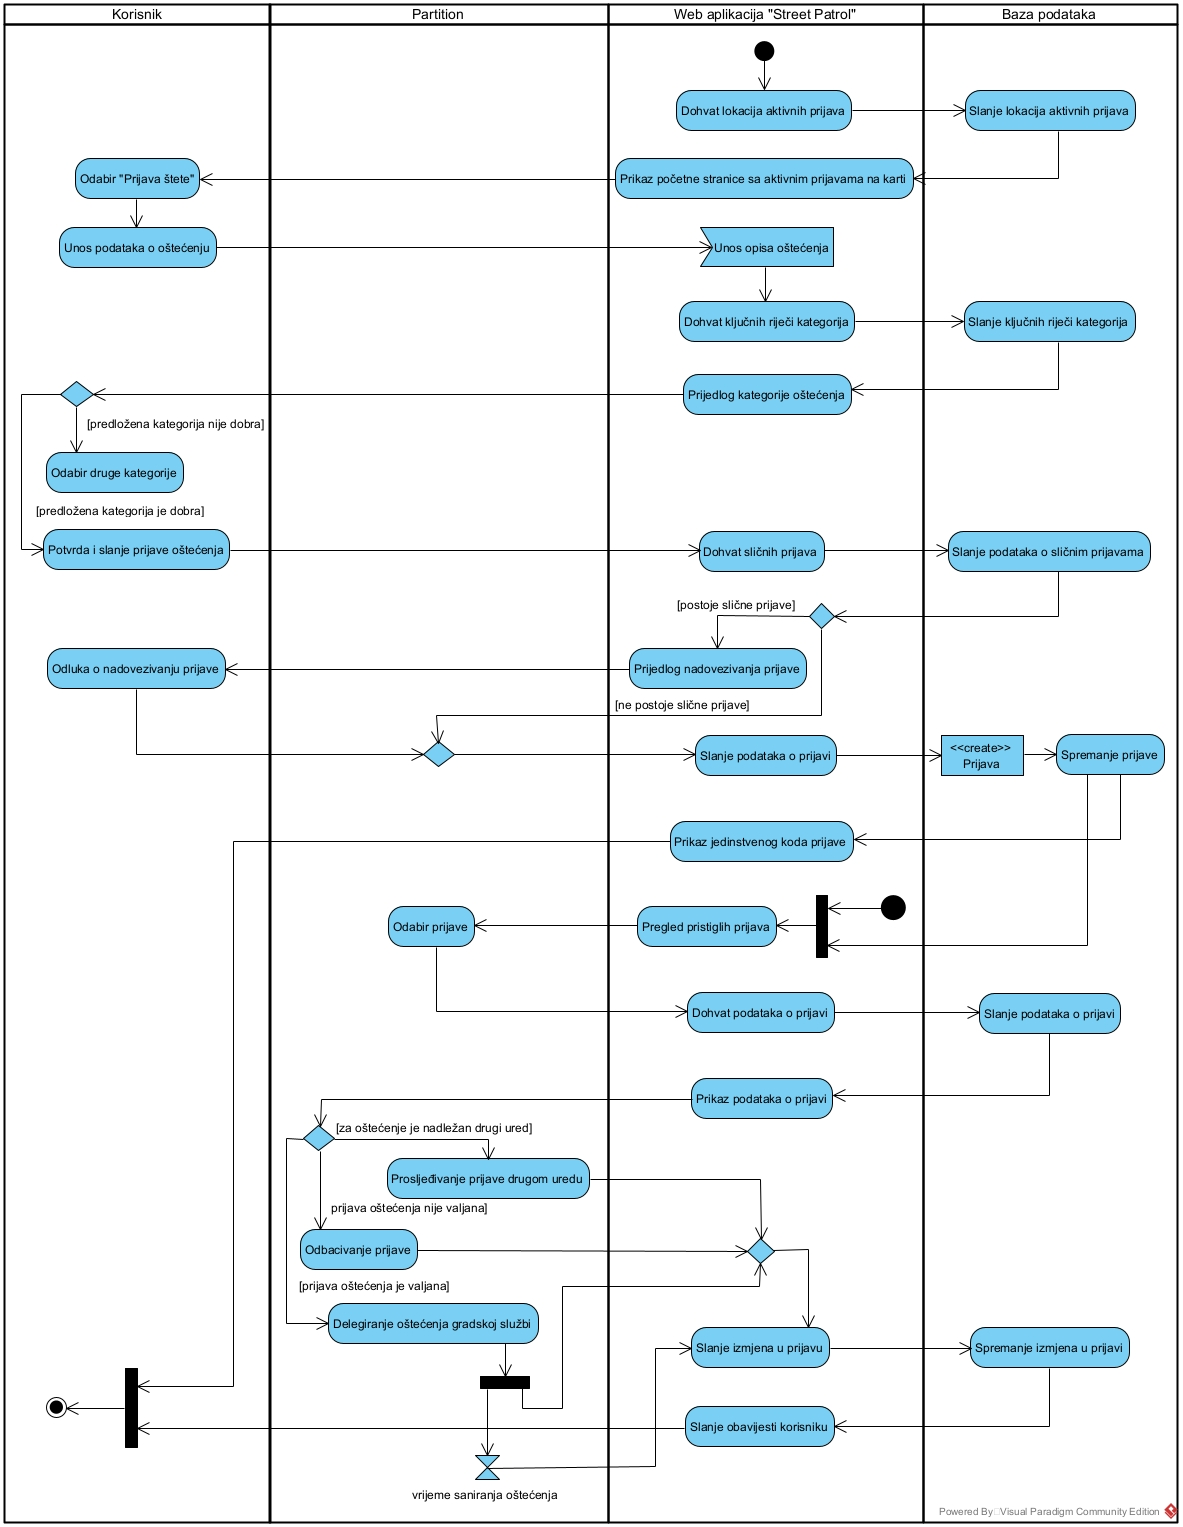
\includegraphics[width=\textwidth]{slike/dijagramAktivnosti.jpg} %veličina u odnosu na širinu linije
				\caption{Dijagram aktivnosti}
				\label{fig:dijagramAktivnosti} %label mora biti drugaciji za svaku sliku
			\end{figure}
			
			\eject
			
			\section{Dijagram komponenti}
			
			\textbf{\textit{dio 2. revizije}}\\
	
			Dijagram komponenti je strukturni statički UML dijagram koji je dio specifikacije arhitekture programske potpore. Njime se vizualizira organizacija i međuovisnost između implementacijskih komponentata i odnos same programske okoline prema okolini. Ovakav tip dijagrama je pogodan kod komponentno-usmjerenog modela razvoja programske potpore i uslužno-orijentirane arhitekture. Osnovni elementi dijagrama komponenti su komponente, sučelja i poveznice.
			
			Na dijagramu \ref{fig:dijagramKomponenti} je prikazana organizacija i međuovisnost komponenata i sučelja u sustavu za prijavu oštećenja na javnim površinama. Dijagram se sastoji od komponente \textit{Web preglednik}, \textit{PostgreSQL baza podataka} i \textit{Web aplikacija}. \textit{Web aplikacija} ima dvije podkomponente: \textit{React frontend} i \textit{Spring Boot backend}. 
			
			Pomoću \textit{Web preglednik} komponente se šalju zahtjevi \textit{Wev aplikacija} komponenti za pojedinim stranicama preko sučelja za dohvat vizualnog sadržaja. \textit{React router} komponenta unutar \textit{React frontend} komponente na temelju URL-a dobivenog od komponente \textit{Web preglednik} donosi odluku koja će se datoteka dohvatiti, to jest koja će se stranica prikazati pomoću komponente \textit{React view}. Komponenta \textit{index.js} je početna komponenta koja služi kao korijen za sve ostale elemente za prikaz. \textit{ReactJS} je biblioteka za sami React. \textit{React view} komponenta po potrebi korisniku osvježava prikaz i preko REST API-ja razmjenjuje podatke sa \textit{Spring Boot backend} komponentom aplikacije u JSON formatu.
			
			\textit{Controller} komponenta unutar \textit{Spring Boot backend} komponente preko REST API-ja prima zahtjeve, šalje ih dalje na obradu i nakon obrade šalje odgovore na njih. \textit{Service} komponenta prima zahtjeve od \textit{Controller} komponente, obrađuje ih i po potrebi komunicira sa \textit{Repository} komponentom. \textit{Repository} komponenta komunicira sa \textit{JpaRepository} komponentom preko JPA sučelja, a \textit{JpaRepository} komponenta preko PSQL sučelja komunicira sa \textit{PostgreSQL baza podataka} komponentom koja služi za trajnu pohranu podataka. \textit{Controller}, \textit{Service} i \textit{Repository} komponente koriste \textit{DTO} komponentu koja služi za enkapsulaciju, organizaciju i razmjenu podataka između komponenti.
			
			\begin{figure}[H]
				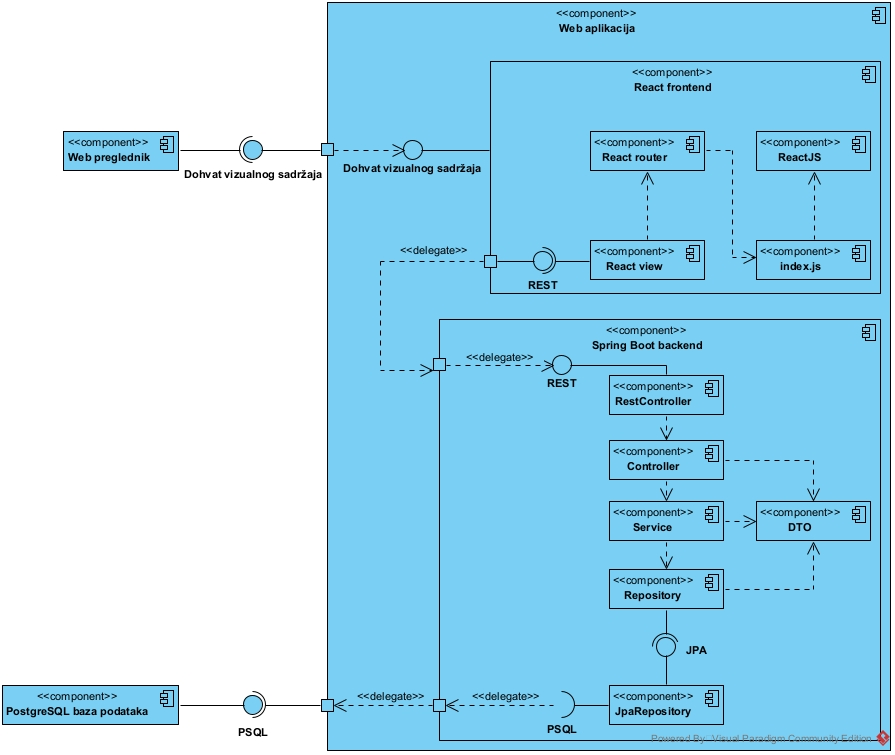
\includegraphics[width=\textwidth]{slike/dijagramKomponenti.jpg} %veličina u odnosu na širinu linije
				\caption{Dijagram komponenti}
				\label{fig:dijagramKomponenti} %label mora biti drugaciji za svaku sliku
			\end{figure}
			
			
			
			
			
			
			
			
			
			
			
			
			